\documentclass[a4paper,12pt]{article}
\usepackage[utf8]{inputenc}
\usepackage{amssymb,amsmath,uniinput,graphicx,hyperref, multirow,units}
\usepackage[section]{placeins}
\usepackage[ngerman]{babel}
\usepackage[left=3cm,right=3cm,top=3cm,bottom=3cm]{geometry}
\renewcommand{\familydefault}{\sfdefault}
\setlength{\belowcaptionskip}{6pt}
\hypersetup{pdfinfo = {
	Title={Versuchsprotokoll zur Paulschen Teilchenfalle},
	Author={Knut Kiesel, Tobias Pook},
	Keywords={Teilchenfalle}
}}


\graphicspath{ {../pictures/} }
\title{Laborpraktikum Teilchenphysik\\ Paulsche Teilchenfalle}
\author{Knut Kiesel\\Tobias Pook}
\date{\today}

\begin{document}
\maketitle
\vspace{5cm}
\tableofcontents
\thispagestyle{empty}
\newpage
\setcounter{page}{1}

\section{Ziel der Messung}
Ziel des Versuchs ist die Speicherung von elektrisch geladenen Teilchen und die Bestimmung des Verhältnisses von Ladung zu Masse.
Um die Teilchen in einem räumlich begrenzten Feld zu halten, ist ein statisches elektrisches Feld nicht ausreichend, da man damit keine Potentialminima schaffen kann.
Eine Möglichkeit dennoch Teilchen zu fangen, ist das Anlegen von phasenverschobenen Wechselspannungen und Gleichspannungen an einem hohlen Würfel, wobei bei richtiger 
Einstellungen der Spannungen und Frequenzen die Teilchen stabil in der Falle bleiben.
Konkret wurden beim durchgeführten Experiment der meta-stabile Bereich eines rotierenden Sattelpotentials genutzt, um Teilchen zu speichern.
Für jede räumliche Komponente $i\in\{x,y,z\}$ lautet die Bewegungsgleichung
\begin{align}\label{mastergleichung}
	\frac{4}{mΩ^2} |\vec{F}_i| + \left( a_i -2q_i \cos\left( 2\xi_i \right) \right) i  + 2k_L \frac{dx}{d\xi_i} + \frac{d^2x}{d\xi_i^2} = B\cos\left( \frac{2ω_W}{Ω}ξ_i \right)
\end{align}
mit den gleichstromabhängigen Koeffizienten $a_i = \frac{16KqU_{G,i}}{3Ω^2mr_0^2}$,
den wechselstromabhängigen Koeffizienten  $q_i = -\frac{4kqU_i}{Ω^2mr_0^2}$,
dem Antriebskoeffienzent $B = \frac{2qU_W}{r_0mΩ^2}$,
dem Luftreibungskoeffizient $k_L = \frac{6πηR}{mΩ}$, der Winkelfrequenz der Dreiphasenspannung $Ω$,
der Winkelfrequenz der zusätzlich an einem Plattenpaar angelegten Wechselspannung $ω_W$
und der normalisierten Zeit $ξ_i = \frac{Ωt}{2} + \frac{iπ}{3}$.
$\vec{F}$ ist eine konstante äußere Kraft, zum Beispiel bei der z-Komponente die Gewichtskraft.
Die Grundschwingung der Lösung wird durch
\begin{align}\label{eq:beta}
β_i = \sqrt{a_i + \frac{q_i^2}{2}}
\end{align}
beschrieben und ist wie auch die Gesamtlösung unabhängig von den Anfangsbedinungen.
Durch Anlegen geeigneter Frequenzen und Spannungen und das Beobachten der entstehenden Teilchenbewegungen kann mit unterschiedlichen Methoden das Verhältnis von Ladung zur Masse bestimmt werden.


\section{Aufbau und Durchführung}
Das Koordinatensystem ist wie folgt definiert:
Die z-Achse verläuft vertikal, die y-Achse ist die Blickrichtung und die x-Achse liegt senkrecht zu den beiden übrigen.

Die Falle wird aus sechs Kupferringen und 12 Verbindungsstücken zu einem Würfel geklebt.
Nach dem Anlöten und Isolieren der Anschlusskabel wird die Falle mit schwarzem Lack angestrichen, um Steulicht in der Kammer zu verringern.
Die Falle wird mittig über der Öffnung für die zur Teilcheninjektion notwendigen Spritze an den Anschlusskabeln befestigt 
und die Plattform von unten an die Spannungsversorgung angeschlossen (siehe Abbildung \ref{fallenbild}),
welche je nach Hebelstellung die Gleichspannungen oder die zusätzliche Wechselspannung zur Dreiphasenspannung hinzufügt.
Die Dreiphasenspannung, im folgenden auch Fokussierspannung genannt, wird aus drei Wechselpannungsquellen, die mit einem konstanten Phasenunterschied von $120^\circ$ betrieben werden, geliefert (siehe Abbildung \ref{verschaltung3phase}).
Die Amplitude kann dabei für jedes Flächenpaar individuell eingestellt werden.

\begin{figure}[htb]
		\centering
		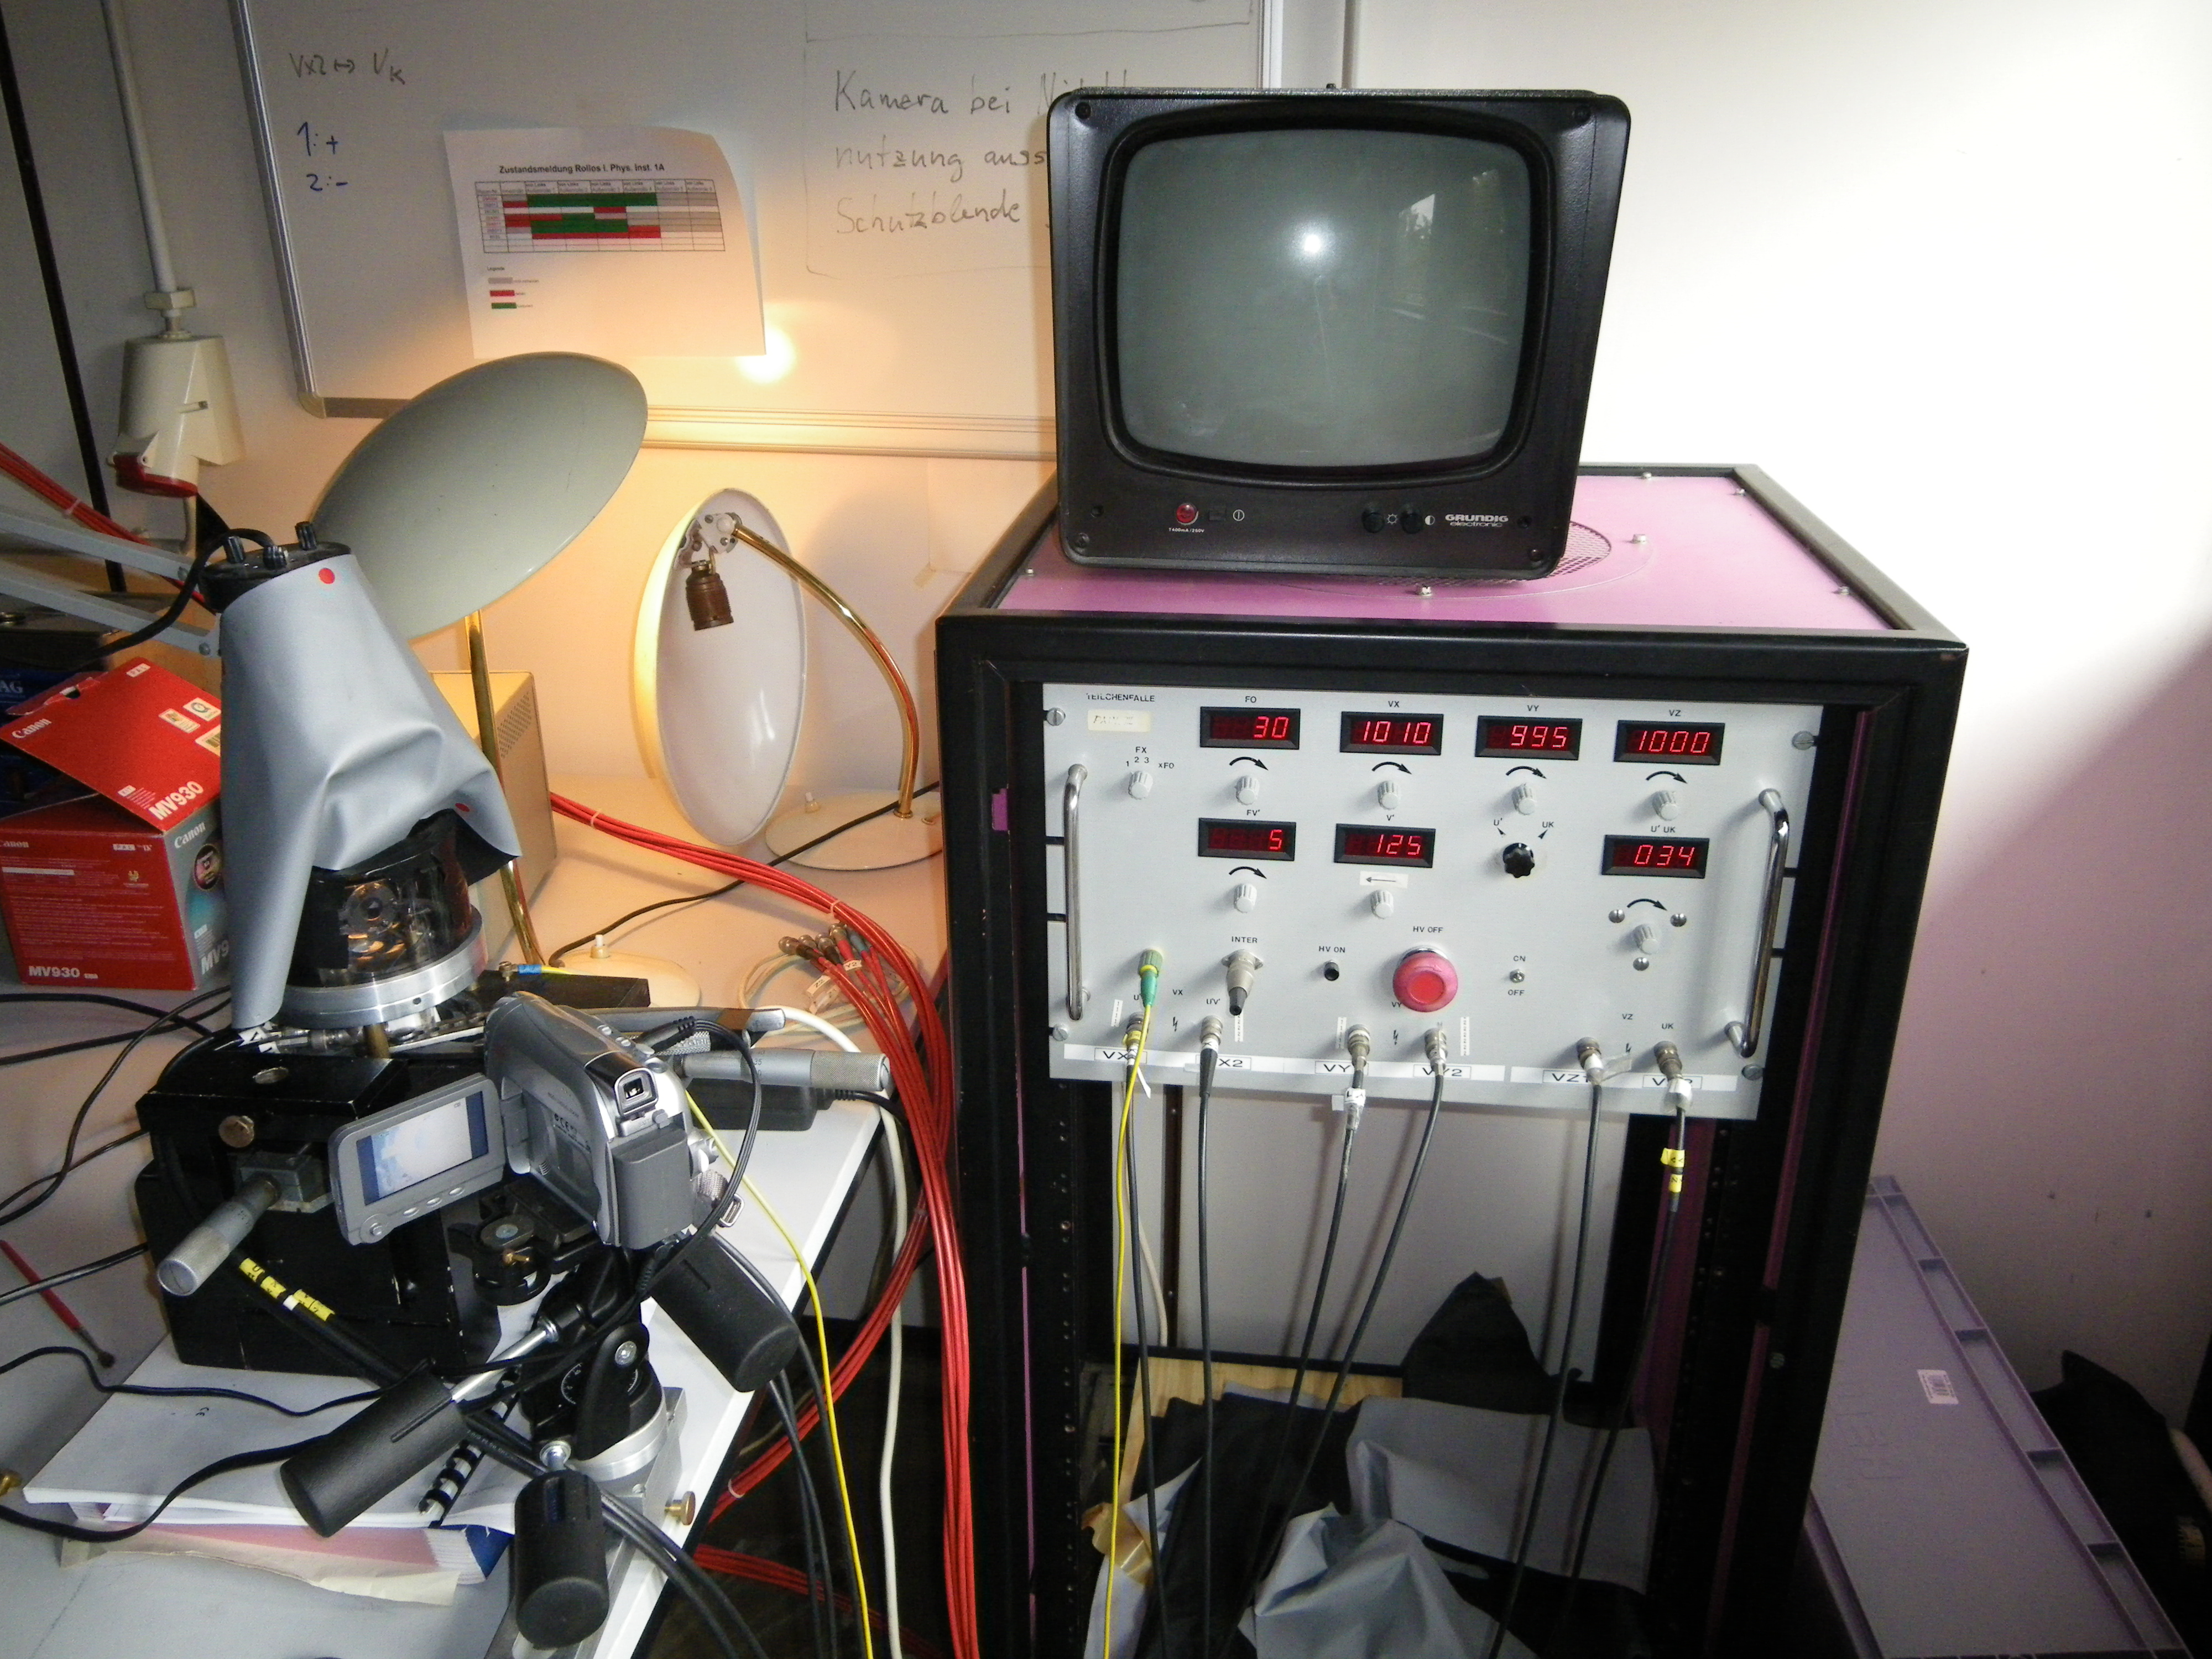
\includegraphics[width=0.8\textwidth]{aufbau.jpg}
		\caption{Versuchsaufbau der Paulschen Teilchenfalle.
			Rechts ist die Spannunsquelle, die mit sechs Kabeln und einer Erdung an die Teilchenfalle (links) angeschlossen ist.
			Vor der Teilchenfalle ist eine Kamera montiert, deren Aufnahme man am Monitor über der Spannungsquelle sehen kann.
			Über der Teilchenfalle ist eine Lampe mit Streulichtschutz angebracht, um die Falle von oben zu beleuchten.
		}
		\label{fallenbild}
\end{figure}

Es gibt mehrere Möglichkeiten die Gleichspannung anzulegen:
Man kann sie auf den beiden gegenüber liegenden Seiten (siehe Abbildung \ref{verschaltungstab}) anlegen, um den gleichstromabhängigen Koeffizienten zu ändern
oder zwischen zwei gegenüberliegenden Seiten (siehe Abbildung \ref{verschaltungz}) anbringen, um eine zusätzliche Kraft $\vec{F}$ ausüben zu können.
Die Wechselspannung wird zwischen zwei gegenüberliegenden Flächen angelegt (siehe Abbildung \ref{verschaltungres}), Frequenz und Amplitude sind einzeln regelbar.
Die Verschaltung ist jedoch schon vorgefertigt und kann mit Schaltern hinzugeschaltet werden.

\begin{figure}[htb]
		\centering
		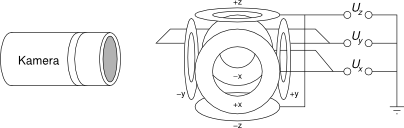
\includegraphics{Schaltbild_3Phasen.png}
		\caption{Verschaltung im Generator für die Fokussierspannung.\cite{versuchsanleitung}}
		\label{verschaltung3phase}
\end{figure}

\begin{figure}[htb]
		\centering
		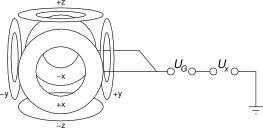
\includegraphics{Schaltbild_Stabilitaet.png}
		\caption{Verschaltung im Generator für eine Gleichspannung auf zwei Flächen um Einfluss auf den gleichstromabhängigen Koeffizienten zu nehmen.
			Diese Spannung kann zur Fokussierspannung hinzugeschaltet werden.\cite{versuchsanleitung}
		}
		\label{verschaltungstab}
\end{figure}

\begin{figure}[htb]
		\centering
		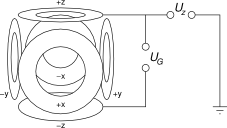
\includegraphics{Schaltbild_Z_Kompensation.png}
		\caption{Verschaltung im Generator für die Gleichspannung zwischen zwei Flächen um eine konstante Kraft in eine Richtung zu erzeugen.
			Diese Spannung kann zur Fokussierspannung hinzugeschaltet werden.\cite{versuchsanleitung}
		}
		\label{verschaltungz}
\end{figure}

\begin{figure}[htb]
		\centering
		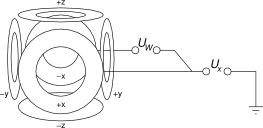
\includegraphics{Schaltbild_Wechselspannung.png}
		\caption{Verschaltung im Generator für die Wechselspannung zwischen zwei Flächen.
			Diese Spannung kann man nicht abschalten, aber auf näherungsweise $0$ regeln.
			\cite{versuchsanleitung}}
		\label{verschaltungres}
\end{figure}

Aus Sicherheitsgründen wird die Falle durch eine durchsichtige Acrylhaube abgedeckt.
Die Haube wurde zusätzlich mit Ausnahme von zwei Stellen mit schwarzem Klebeband verkleidet.
Die zwei Öffnungen dienen der seitlichen Beobachtung der Falle und der Bestrahlung durch eine oben angebrachten Lampe.
Die geladen Teilchen sind Aluminiumpulverstücke, die mittels einer Spritze durch eine Öffnung unterhalb der Falle eingebracht werden.
Wenn die Aluminiumpartikel schnell an der Kanüle der Spritze entlangreiben, werden manche Teilchen ionisiert.
Da zwischen Öffnung und dem stabilen Bereich der Teilchenfalle ein Abstand von ca. $\unit[2.5]{cm}$  besteht,
 wurden die Teilchen durch Anschnipsen der Spritze in die Falle geschleudert, um einerseits die Richtige Höhe zu haben und anderseits genug Ladung an der Spritzenspitze abzugeben.

Zusätzlich zum Messaufbau in Luft gibt es noch einen zweiten Messaufbau für Versuche im Vakuum.
Hier befindet sich eine baugleiche Falle in einer zylindrischen, mit Scheiben versehenen Vakuumkammer.
Die Kammer besitzt mehrere Öffnungen, an denen Beobachtungsfenster,Stromversorgung,Vakuumpumpe und ein beweglicher Hebel mit Halterung für die Spritze luftdicht angebracht werden können.
Da während der Versuchsdurchführung die Vakuumpumpe defekt war,
konnten Messungen lediglich bei vermindertem Luftdruck, im Bereich zwischen $\unit[300]{mbar}$ und $\unit[450]{mbar}$ durchgeführt werden.

Es gibt auch eine vorgefertigte Falle, die sich in einer Vakuumkammer befindet.
Diese kann man mit einer Turbinenpumpe und bei niedrigeren Drücken mit einer Turbo-Molekularpumpe evakuieren und den Druck mithilfe eines Drucksensors überprüfen.

\subsection*{Technische Probleme des Versuchsaufbau}
Der genutzte Versuchsaufbau hat während der Messungen eine Reihe von technischen Problemen aufgewiesen die im folgenden kurz erläutert werden.Der Einfluss
auf die durchgeführten Messungen wird bei der Auswertung der verschiedenen Messreihen im Kapitel \ref{Ergebnisse} behandelt.
\subsubsection*{Schwankungen der Fokussierspanung}
Die Amplitude der Dreiphasenspannung unterlag starken Schwankungen, diese lassen sich in drei Kategorien eingeteilt werden:
\begin{itemize}
\item
Schwankungen im Bereich von \unit[±15.0]{V} bis \unit[±50.0]{V} um einem konstanten Mittelwert.
\item
Kontinuierliches ansteigen der Fokussierspannung zwischen dem Flächenpaar in y-Richtung von etwa $\unit[1400]{V}$ bis $\unit[3000]{V}$ gefolgt von einem plötzlich
Abfall zurück auf $\unit[1400]{V}$. Die Spannung lässt sich dann praktisch nicht mehr durch den zugehörigen Drehschalter beeinflussen.
\item
Plötzlicher Abfall der Fokussierspannung für das Flächenpaar in x-Richtung von der gewählten Spannung auf ca. $\unit[200]{V} - \unit[300]{V}$ und daraus resultierender
Verlust der Teilchen.
\end{itemize}
Für die beiden letzten Probleme wird mangelnde Kühlung der Hochspannungsquelle als Grund vermutet, da die Fehlfunktion nach längerem ausschalten des Gerät zunächst nicht mehr auftritt.

\subsubsection*{Fangen von Teilchen im Vakuum}
Beim Evakuieren der Kammer kann der gewünschte Druck von einigen $\unit{μbar}$ nicht erreicht werden.
Die Frontanzeige 1liefert bei Erreichen von $90μbar$ einen Fehlercode und auch auf der Rückseite des Sensors ist der Druck immer noch zu groß.
Auch das Halten von Teilchen in der Falle gestaltet sich bei diesen Einstellungen als schwierig, man kann erahnen wie die Teilchen immer zu einer Seite abgesaugt werden.
Grund dafür könnte ein Leck an der Vakuumkammer sein, ein Defekt der Turbo-Molekularpumpe ist aber auch nicht ausgeschlossen.
Da das Saugen der Pumpe jede Speicherung während des Pumpens unmöglich macht, ist die einzige Möglichkeit, Teilchen in der Vakuumfalle zu halten, die Pumpe auszuschalten.
Der Druck fällt rasch auf ein paar $\unit[100] {mbar}$ ab und ist dann relativ stabil, was einem das Einfangen von Teilchen erlaubt.

\section{Ergebnisse}\label{Ergebnisse}
Mit einem Messschieber wird der Plattenabstand der Teilchenfalle auf $2r_0 = d = \unit[(3.05±0.02)]{cm}$ abgeschätzt.
\subsection{Bahnbeschreibung}
Obwohl die Bahnkurven unabhängig von den Anfangsbedinungen sein sollten, lassen sich nur die wenigsten Teilchen fangen.
In den meisten Fällen beschreiben die eingefangenen Teilchen eine elliptische Teilchenbahn, deren Radius und die Exzentrizität durch das Verhältnis der angelegten Potenziale 
in der Fokusierspannung erklärt werden können.
Viele Teilchen beschreiben zudem sehr kleine Bahnen und sind deshalb nur noch als Punkte wahrzunehmen.

\subsubsection*{Lissajous Figuren}
In einigen Fällen können sich auch Lissajous Figuren bilden. Lissajous Figuren entstehen bei der Überlagerung harmonischer Schwingungen, wenn das Verhältnis der Frequenzen rational ist.
In diesem Fall bildet die Teilchenbahn eine geschlossene Figur.
Die möglichen Formen der Figuren sind sehr vielfältig und hängen vom Frequenzverhältnis und dem Phasenunterschied der Schwingungen ab.
Ein Beispiel einer spiralförmigen Figur ist in Abbildung \ref{Lissjous} zu sehen.

\begin{figure}[htb]
		\centering
		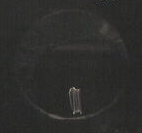
\includegraphics{lisa_klein.jpg}
		\caption{Beispiel für das Auftreten einer Lissajous Figur in der Paulschen Teilchenfalle.
		Das Teilchen beschreibt hier eine spiralähnliche Bahn.}
		\label{Lissjous}
\end{figure}

\subsubsection*{Kristallstruktur}
Wenn man mehrere Teilchen in der Teilchenfalle gefangen hat, kann man manchmal Pseudo-Kristallstrukturen erkennen:
Die Teilchen stoßen sich gegenseitig ab und suchen energetisch günstige Zustände, ebenso wie in einem Kristall.
Überlagert zu diesem Effekt sieht man in Abbildung \ref{pseudokristall} noch die Auswirkungen des Feldes.
In der hier sichtbaren $x = 0$ und $z = 0$  Ebene werden keine Teilchen gehalten, wie man auch Gleichung (\ref{mastergleichung}) entnehmen kann.
%Da man im Vakuum Teilchen besser fangen kann (siehe nächsten Abschnitt), werden im Vakuum mehr Teilchen gleichzeitig gefangen, und man kann die Strukturen besser sehen.

\begin{figure}[htb]
		\centering
		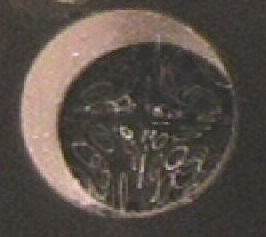
\includegraphics{pseudo_kristall.png}
		\caption{Beispiel zur Pseudokristallstruktur im Vakuum. Im Hintergrund ist als heller Halbmond die hintere angeleuchtete Ringscheibe zu sehen.}
		\label{pseudokristall}
\end{figure}


\subsection{Kompensation der Gewichtskraft}\label{sec:kompensation}
In Gleichung (\ref{mastergleichung}) wird der Einfluss der Luftreibung vernachlässigt und ein Näherungsansatz der Form $z(ξ_z) = Z(ξ_z)+d(ξ_z)$ durchgeführt.
Die z-Komponente wird nun durch
\begin{align*}
	Z(ξ) = Z_0\sin(β_zξ) - \frac{4|\vec{F}_z|}{mβ_zΩ^2}
\end{align*}
beschrieben.
Man sieht, dass die Schwingung um einen konstanten Term verschoben ist, der von $a_z$ und $q_z$ abhängt.
Diese Abhängigkeit besteht nicht mehr, wenn gilt:
\begin{align}
	\label{kraftgleichgew}
	|\vec{F}_{z}| = |\vec{F}_G + \vec{F}_{qE}| = mg + q\frac{U_G}{d} = 0
\end{align}

Zu der Dreiphasenspannung wird nun ein zusätzlicher Potentialunterschied zwischen den beiden z-Komponenten angeschlossen (siehe Schaltplan in Abbildung \ref{verschaltungz}), der solange erhöht wird,
 bis die Gravitationskraft kompensiert wird.
Dies kann dadurch überprüft werden, dass sich der Mittelpunkt der Teilchenschwingung bei Änderung der Amplitude der z-Komponente der Dreiphasenspannung nicht mehr ändert.
Die Fokussierspannung wird bei $U_i = \unit[(1414±14)]{V}$ für alle Flächenpaare betrieben.


Weil die Gleichspannung stark schwankend ist, wird die effektive Spannung durch Notieren der angezeigten Werte in einem Zeitraum von ungefähr $\unit[20]{s}$ und anschliessendem Mitteln bestimmt. 
Der Fehler auf die Stichprobe wird im folgenden "`statistischer"' Fehler genannt.
Da man die Teilchen oft wegen spontaner Spannugsschwankungen der Quelle verliert, kann der Bereich in dem die Gravitationskraft kompensiert wird, nicht in feineren Spannungsabschnitten untersucht werden.
Dies führt dazu, dass nicht abgeschätzt werden kann, wie exakt der Wert für die Kompensationsspannung $U_G$ getroffen wird.
Die mittlere Differenz zu den nächstliegenden $U_G$ Messwerten, bei denen wieder Bewegungen des Schwingungsmittelpunkt bei Variation der Fokussierspannung $U_z$ zu beobachten sind,
wird deshalb "`systematischer"' Fehler genannt.
Die Messungen werden teilweise für mehrere gleichzeitig gefangene Teilchen durchgeführt und die Spannung erhöht bis alle Teilchen den Stabilitätsbereich verlassen haben. Die Messergebnisse sind in
Tabelle \ref{tab:z-komp-measure} aufgeführt, dabei werden für die einzelnen Messungen unterschiedliche Teilchen benutzt. Es wurde zusätzlich eine Messung unter vermindertem Luftdruck von
 $\unit[(450±50)]{mbar}$ durchgeführt.
Das Vorzeichen der Ladung ergibt sich aus dem Anschluss an die Spannungsquelle und ist für alle beobachteten Teilchen negativ, was mit der Theorie übereinstimmt.

\begin{table}[h]
	\centering
	\begin{tabular}{ l|c | c | l | l }
		Messung  & $U_{G} [V]$ & $\sigma_{U_{G}}[V]$ & \multicolumn{2}{l}{Verhalten bei Änderung von $U_z$}\\
		\hline
		\hline
		\multirow{5}{*}{I (2 Teilchen)}&45 & 5 & Bewegung &  Bewegung   \\
		&92 & 8 & still  & Bewegung \\
		&168 & 4 & Bewegung & Bewegung    \\
		&228 & 3 & Bewegung & Bewegung \\
		&273 & 5 & verloren & still \\
		\hline
		\multirow{4}{*}{II}&33 & 5 & Bewegung \\
		&50 & 4 & still\\
		&60 & 5 & Bewegung \\
		&79 & 7 & Bewegung\\
		\hline
		\multirow{3}{*}{III (Vakuum)*}&25 & 3 & Bewegung\\
		&68 & 3 & still\\
		&79 & 7 & Bewegung\\
	\end{tabular}
	\caption{Verhalten des Bahnmittelpunkts von Teilchen  bei unterschiedlichen Gleichspannungen zur Bestimmung der z-Kompensation.\newline
		*: Messung III wurde unter vermindertem Luftdruck von $p = \unit[(450±50)]{mbar}$ durchgeführt.
	}
	\label{tab:z-komp-measure}
\end{table}

Aus Gleichung \ref{kraftgleichgew} lässt sich direkt eine Formel für die spezifische Ladung des untersuchten Teilchen herleiten:
\begin{align}\label{zspezm}
	\frac{q}{m} = -\frac{g \cdot  d}{U_{G}}
\end{align}
Die berechneten Werte können Tabelle \ref{tab:z-komp-result} entnommen werden. Hierbei wird die Erdbeschleunigung 
$g = \unitfrac[(9.81)]{m}{s^2}$ als konstant (fehlerfrei) angenommen und die Unsicherheit auf den Fallendurchmesser als weitere
% wollen wir da wirklich konstant schreiben? ok, auch recht
unabhängige systematische Fehlerquelle betrachtet.


\begin{table}[h]
	\centering
	\begin{tabular}{ c | c }
		$U_{G,komp} [V] $ & $-\frac{q}{m}[\frac{mC}{kg}]$ \\
		\hline
		  68 ± 3(stat.) ± 27(sys.) &  4.40 ± 0.16(stat.) ± 1.76(sys.)  \\
		  50 ± 4(stat.) ± 14(sys.) &  5.95 ± 0.53(stat.) ± 1.67(sys.)  \\
		  92 ± 8(stat.) ± 62(sys.) &  3.27 ± 0.28(stat.) ± 2.21(sys.)  \\
		  273 ± 5(stat.) ± 55(sys.) & 1.09 ± 0.02(stat.) ± 0.23(sys.)  \\
	\end{tabular}
	\caption{Die Kompensationsspannung und das das daraus resultierende Verhältnis von Ladung zu Masse von verschiedenen Teichen}
	\label{tab:z-komp-result}
\end{table}


Alle Messwerte liegen in einem mit einander kompatiblen Wertebereich. Durch die hohen systematischen Unsicherheiten auf das
Treffen der richtigen Kompensationsspannung entstehen relative Unsicherheiten im Bereich von $20\% - 70 \%$. Die erzeugten
Ergebnisse bieten also nur die Möglichkeit grob die Größenordnung der spezifischen Ladungen von Teilchen zu bestimmen.

\subsection{Resonanz}
In diesem Versuchsteil wird zusätzlich zur Fokusierspannung eine Wechselspannung zwischen dem Flächenpaar entlang der x-Achse angelegt.
Die Gleichspannung wird auf $0$ geregelt.

Bei einer Frequenz von
\begin{align}\label{w_res}
	\omega^{res}_W = \frac{\Omega}{2}\sqrt{\beta^{2}_x-2k^{2}_L}
\end{align}
tritt eine resonante Verstärkung der Oszillation auf und die Teilchenbahn erreicht ihre maximale Auslenkung
\begin{align}\label{Amax}
	A_{max} = \frac{B}{2k_L\sqrt{\beta^{2}_x-k^{2}_L}}.
\end{align}
Durch Eliminieren von $k_L$ in Gleichung \ref{w_res} und \ref{Amax} erhält man
\begin{align}\label{res_luft}
	\frac{q}{m}|_{\text{Luft}} = ±\sqrt{
		\frac{
			\left( \frac{U_w}{A_{max}} \right)^2 ± \sqrt{
				\left( \frac{U_w}{A_{max}} \right)^4 + \left( \frac{4KU_xω^{res}_W}{Ω r_0}\right)^4
			} %sqrt
		}{
			32r_0^2\left( \frac{U_xK}{Ωr_0^2} \right)^4
		} % frac
	}. % sqrt
\end{align}
Da das Verhältnis in  alle anderen Versuchen negativ ist, wird auch hier nur das negative Ergebnis betrachtet.
Um radizieren zu können, muss das Vorzeichen unter der Wurzel positiv sein.
Für die Lösung im Vakuum reicht es in Gleichung (\ref{w_res}) $k_L=0$ zu setzen, und man erhält
\begin{align}\label{res_vak}
	\frac{q}{m}|_\text{Vakuum} = -\frac{\Omega r^{2}_0 \omega^{res}_W}{\sqrt{2} K U_x}.
\end{align}

Um die Resonanzfrequenz eines Teilchens zu messen, wird die Wechselspannung variiert bis das Teilchen maximale Auslenkung zeigt.
In Luft wird zusätzlich die maximale Auslenkung $A_{max}$ bestimmt, indem mit einer Digitalkamera Fotos der Teilchenbahn angefertigt werden.

Bei niedriger Fokusierfrequenz erhöht sich der relative Fehler und bei hoher Fokusierfrequenz wird die Stabilitätsgrenze schneller erreicht
, darum wurde eine Winkelfrequenz von $Ω = (503±6)\unit{Hz}$ gewählt.
Die Messungen wurden bei zwei verschiedenen Fokussierspannungen durchgeführt: $\unit[(1414±14)]{V}$ und $\unit[(707±14)]{V}$.
In beiden Konfigurationen wurden jeweils 2 Teilchen in Luft und jeweils 2 im Vakuum vermessen.
Die Amplitude der Wechselspannung unterliegt starken Schwankungen und wird mit einem Wert von
$ \unit[( 210 ± 30 )]{V} $ gemessen, sie lässt sich kaum durch den dafür vorgesehenen Drehschalter regeln.

Der Ausschlag der Teilchen wird über das Verhältnis der Amplitude zum Innendurchmesser der Falle $d_{innen}$ bestimmt und ist für alle 8 Teilchen innerhalb des Fehlers gleich.
$$A_{max} = \frac{A_{max}\text{ [Pixel]}}{d_{innen}\text{ [Pixel]}} \cdot d_{innen}= \unit[( 0.7 ± 0.4 )]{mm} $$
Alle gemessenen Teilchen zeigen ihre maximale Auslenkung bei $\omega_W \leq \unit[(31±6)]{Hz}$,
was die minimal an der Spannungsquelle einstellbare Frequenz ist.

Wenn man die Resonanzfrequenz durch die Grundschwingungsfrequenz in Luft $\bar{ω}_0$ ausdrückt, erhalt man
\begin{align*}
	ω^{res}_W = \sqrt{ \bar{ω}_0^2 - \frac{Ω^2k_L^2}{2} },
\end{align*}
was dazu führt, dass die Resonanz unterhalb der Grundschwingungsfrequenz liegt.
Die beobachteten Ereignisse waren wahrscheinlich keine Schwingungsmaxima, dass heißt die eigentlich gesuchte Frequenz liegt unterhalb der beobachteten.
Schon die Lissajous Figur von Abbildung \ref{Lissjous} hatte eine größere Amplitude.

Um Interpretationsfehler zu vermeiden, wurde dennoch das ganze zur Verfügung gestellte Frequenzspektrum abgefahren, aber ohne eine zusätzliche Resonanz zu entdecken.

Auch die Amplitude blieb bei allen 4 Teilchen in Luft und 4 Teilchen im Vakuum (innerhalb des Fehlers) gleich groß.
Man erhält mit gausscher Fehlerfortplanzung erhält man die Obergrenzen, die in Tabelle \ref{tab:resonanz} dargestellt sind.

\begin{table}[h]
	\centering
	\begin{tabular}{l|c|c}
		$U_x \unit{[V]}$ & $-\frac{q}{m}|_\text{Luft}\unit{\left[\frac{mC}{kg}\right]} $&$-\frac{q}{m}|_\text{Vakuum}\unit{\left[\frac{mC}{kg}\right]}$\\
		\hline
		707 & 0.3 ± 0.1 &  0.17 ± 0.04 \\
		1414 & 0.11 ± 0.03 & 0.09 ± 0.02
	\end{tabular}
	\caption{Die Grenzen der Verhältnisse von Ladung zu Masse bei in Luft und in Vakuum.
		Die Versuche wurden jeweils bei unterschiedlichen Spannungen und jeweils mit zwei Teilchen durchgeführt.}
	\label{tab:resonanz}
\end{table}

Die Werte nehmen mit zunehmender Spannung ab, was auch zu erwarten war.
Für Luft und Vakuum sind die Werte noch  miteinander vereinbar, der Wert in Luft ist immer größer als im Vakuum.
Die relativen Fehler sind alle im Bereich von $20\%$.
Die Unvereinbarkeit der Werte stellt aber  kein Problem dar,
da es nur Obergrenzen sind. Um nicht nur Obergrenzen zu messen,
müsste man eine niedrigere Anregungsfrequenz anlegen, was bei der vorgegebenen
Spannungsquelle nicht möglich ist.


\subsection{Stabilitätsdiagramm}
Die Grundschwingung in Gleichung (\ref{eq:beta}) muss real sein, da sonst die Winkelfunktionen zu Expotentialfunktionen werde, was zum Austritt der Teilchen aus der Falle führt.
Hier wird nur der Grenzfall $β_x = a + \frac12q^2  =0$ untersucht.
Dafür wird bei verschiedenen, konstanten $U_x = U_y = U_z = U_i$ die an der x-Achse angelegten Gleichsannung $U_G$ gesucht, bei der das Teilchen entkommt.
Weil das Teilchen nicht entkommen darf (es muss bei mehreren $U_i$ vermessen werden), ist die Abschätzung nur schwer zu bewerkstelligen, da die Gleichspannungsquelle stark schwankt 
und es somit leicht entkommen kann.
Dies führt zu einem systematischen Fehler in $U_G$.
Für jedes Teilchen wird bei konstantem $Ω =\unit[188±6]{Hz}$ die Gleichspannung $U_g$ gegen $U_i^2$ aufgetragen und eine lineare Regression durchgeführt.
Die Anpassungen sind in Abbildung \ref{linReg} zu sehen.
\begin{figure}[htb]
		\centering
		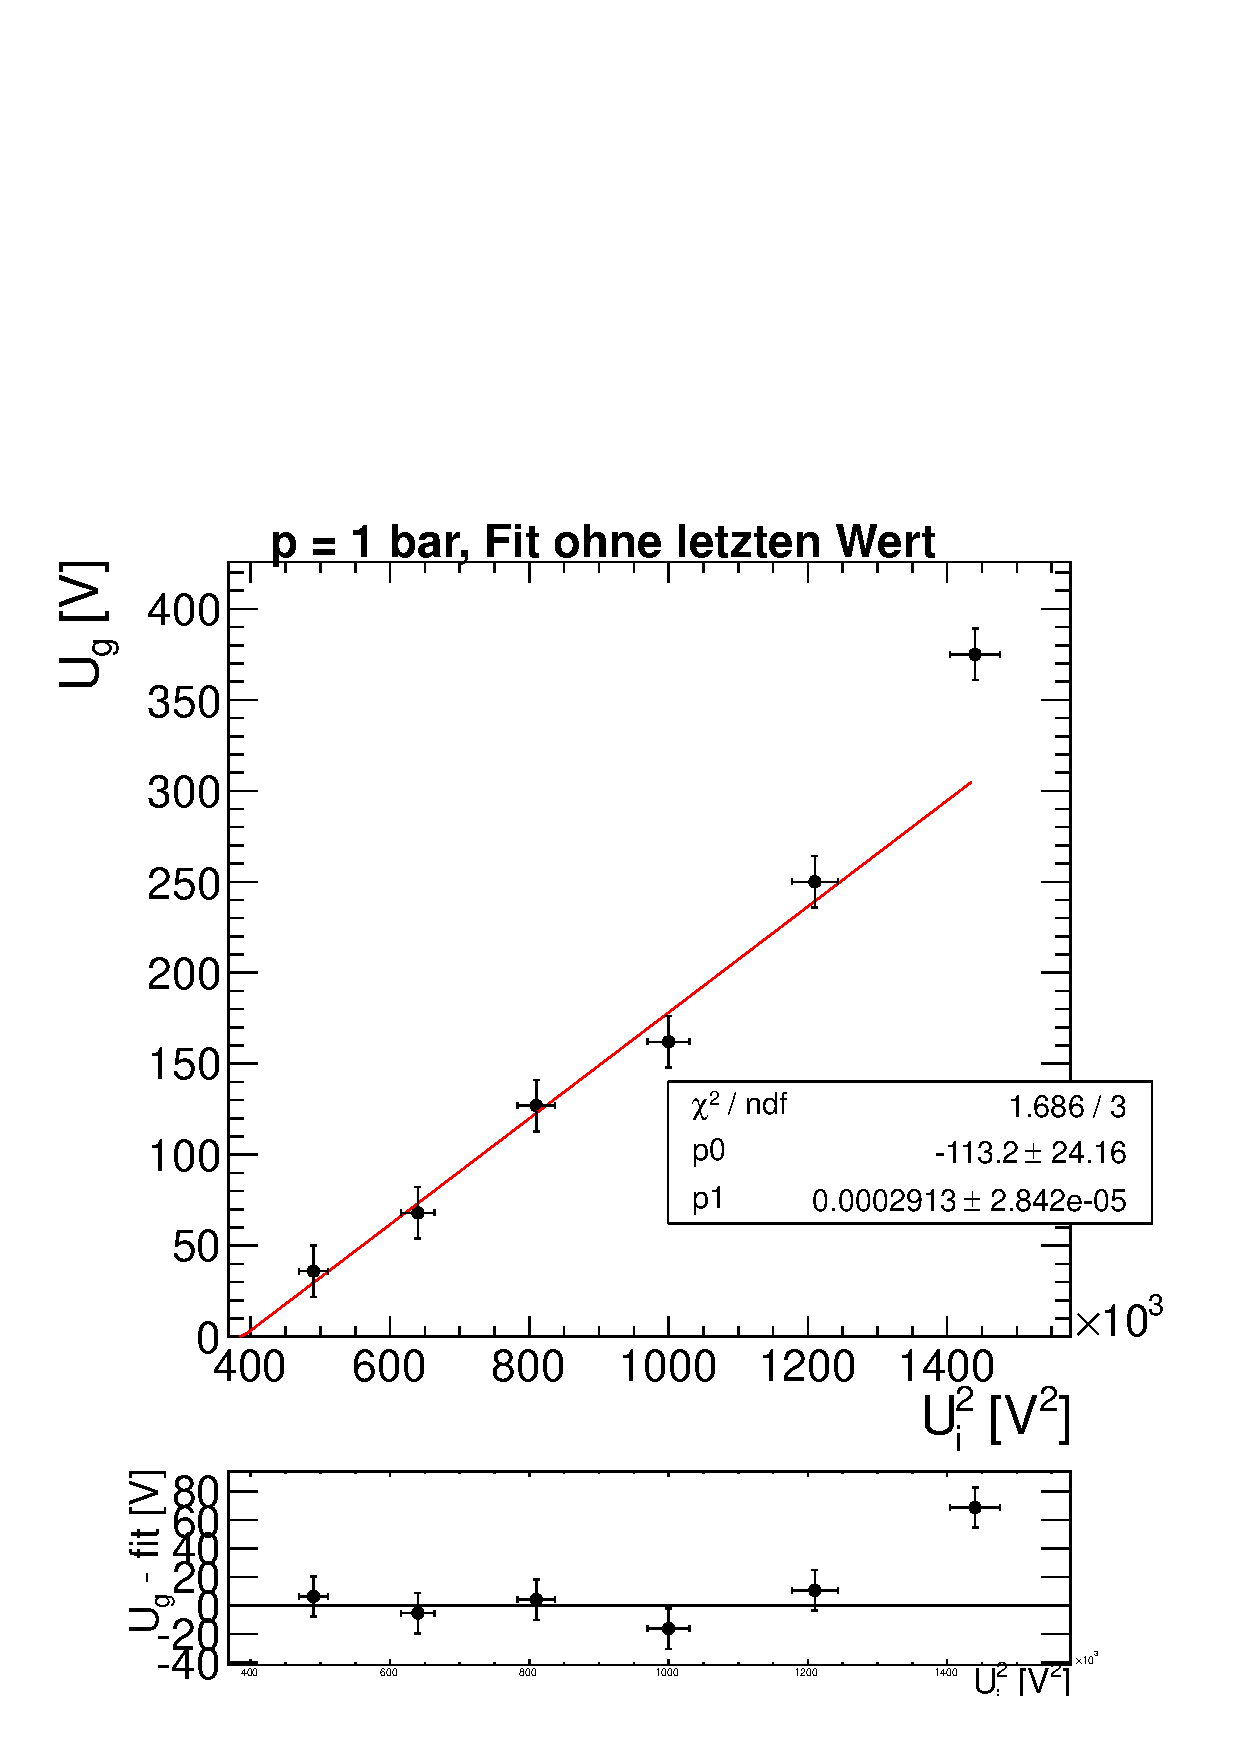
\includegraphics[height = 0.3\textheight]{linRegLuft1.pdf}
		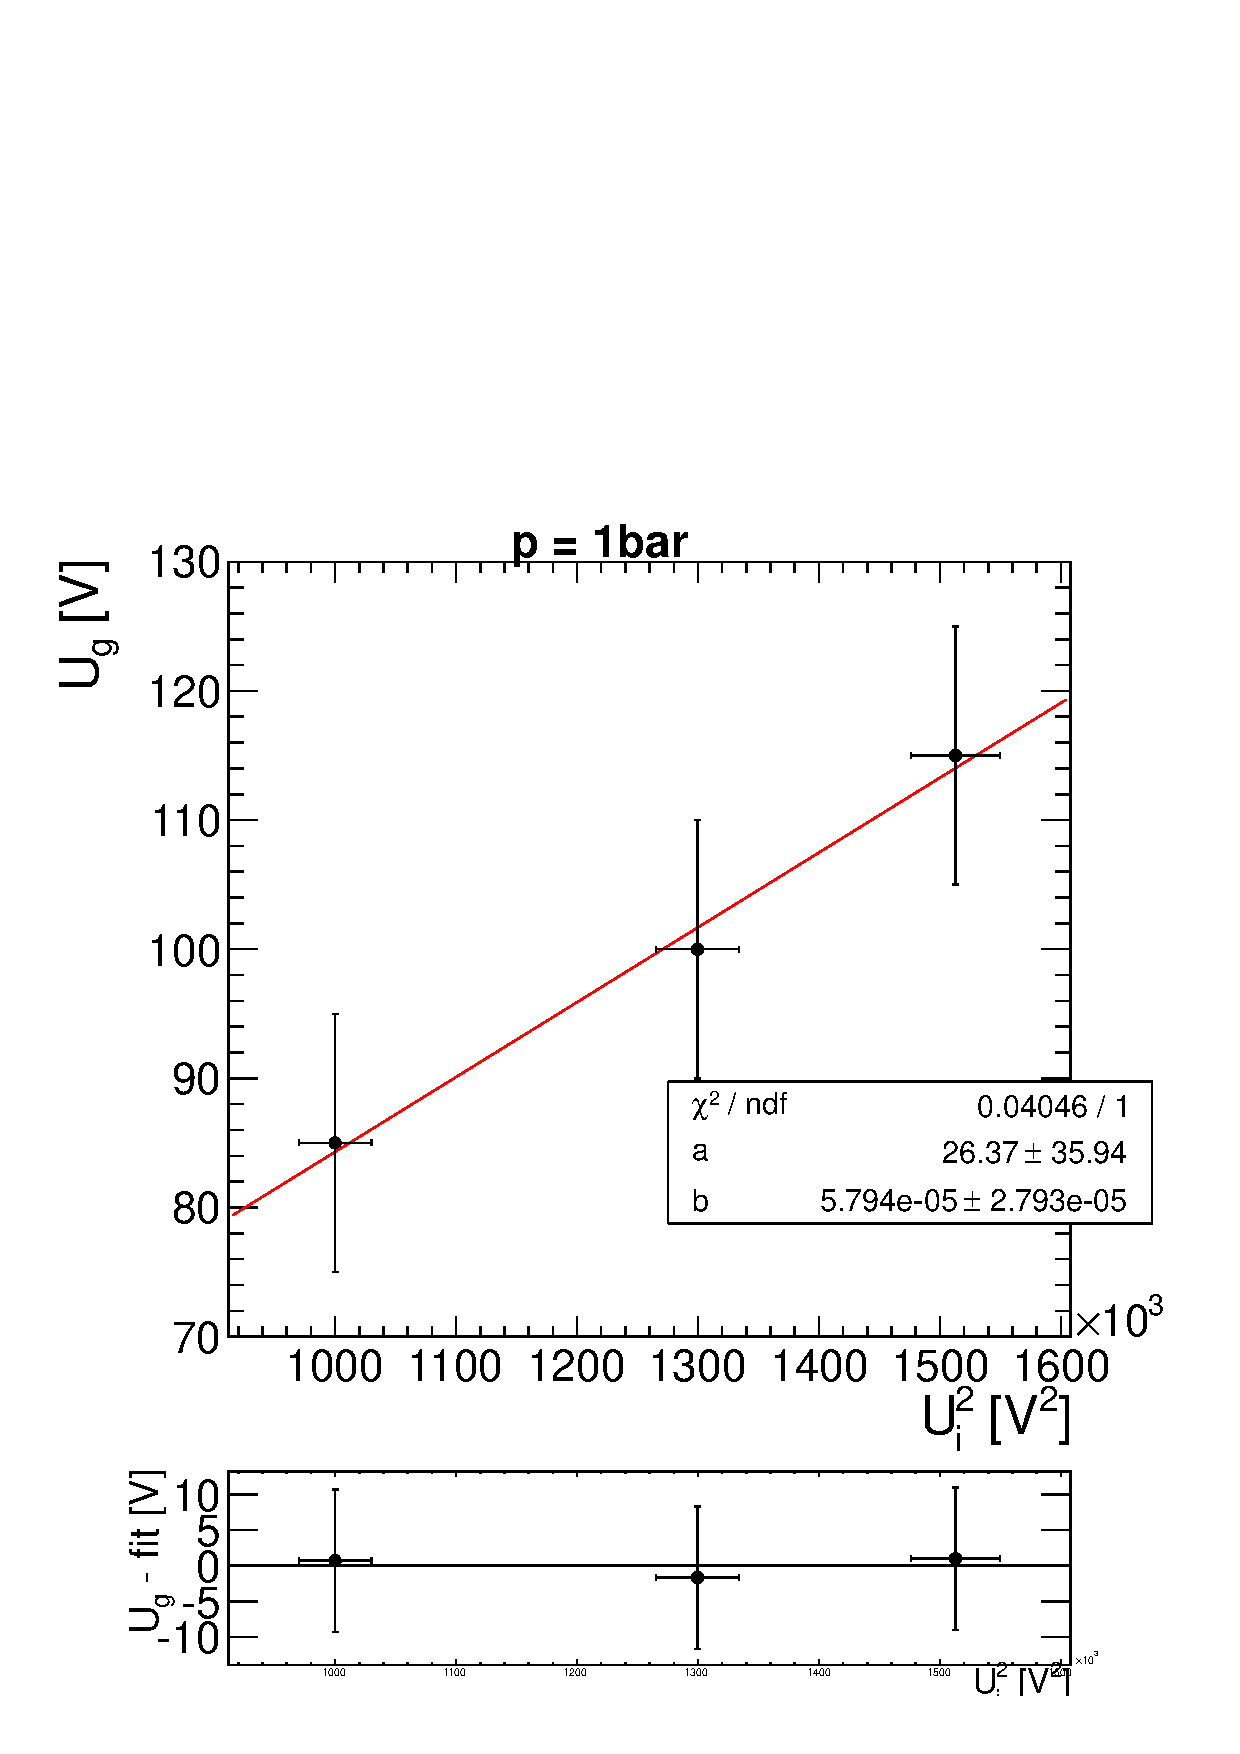
\includegraphics[height = 0.3\textheight]{linRegLuft2.pdf}\\
		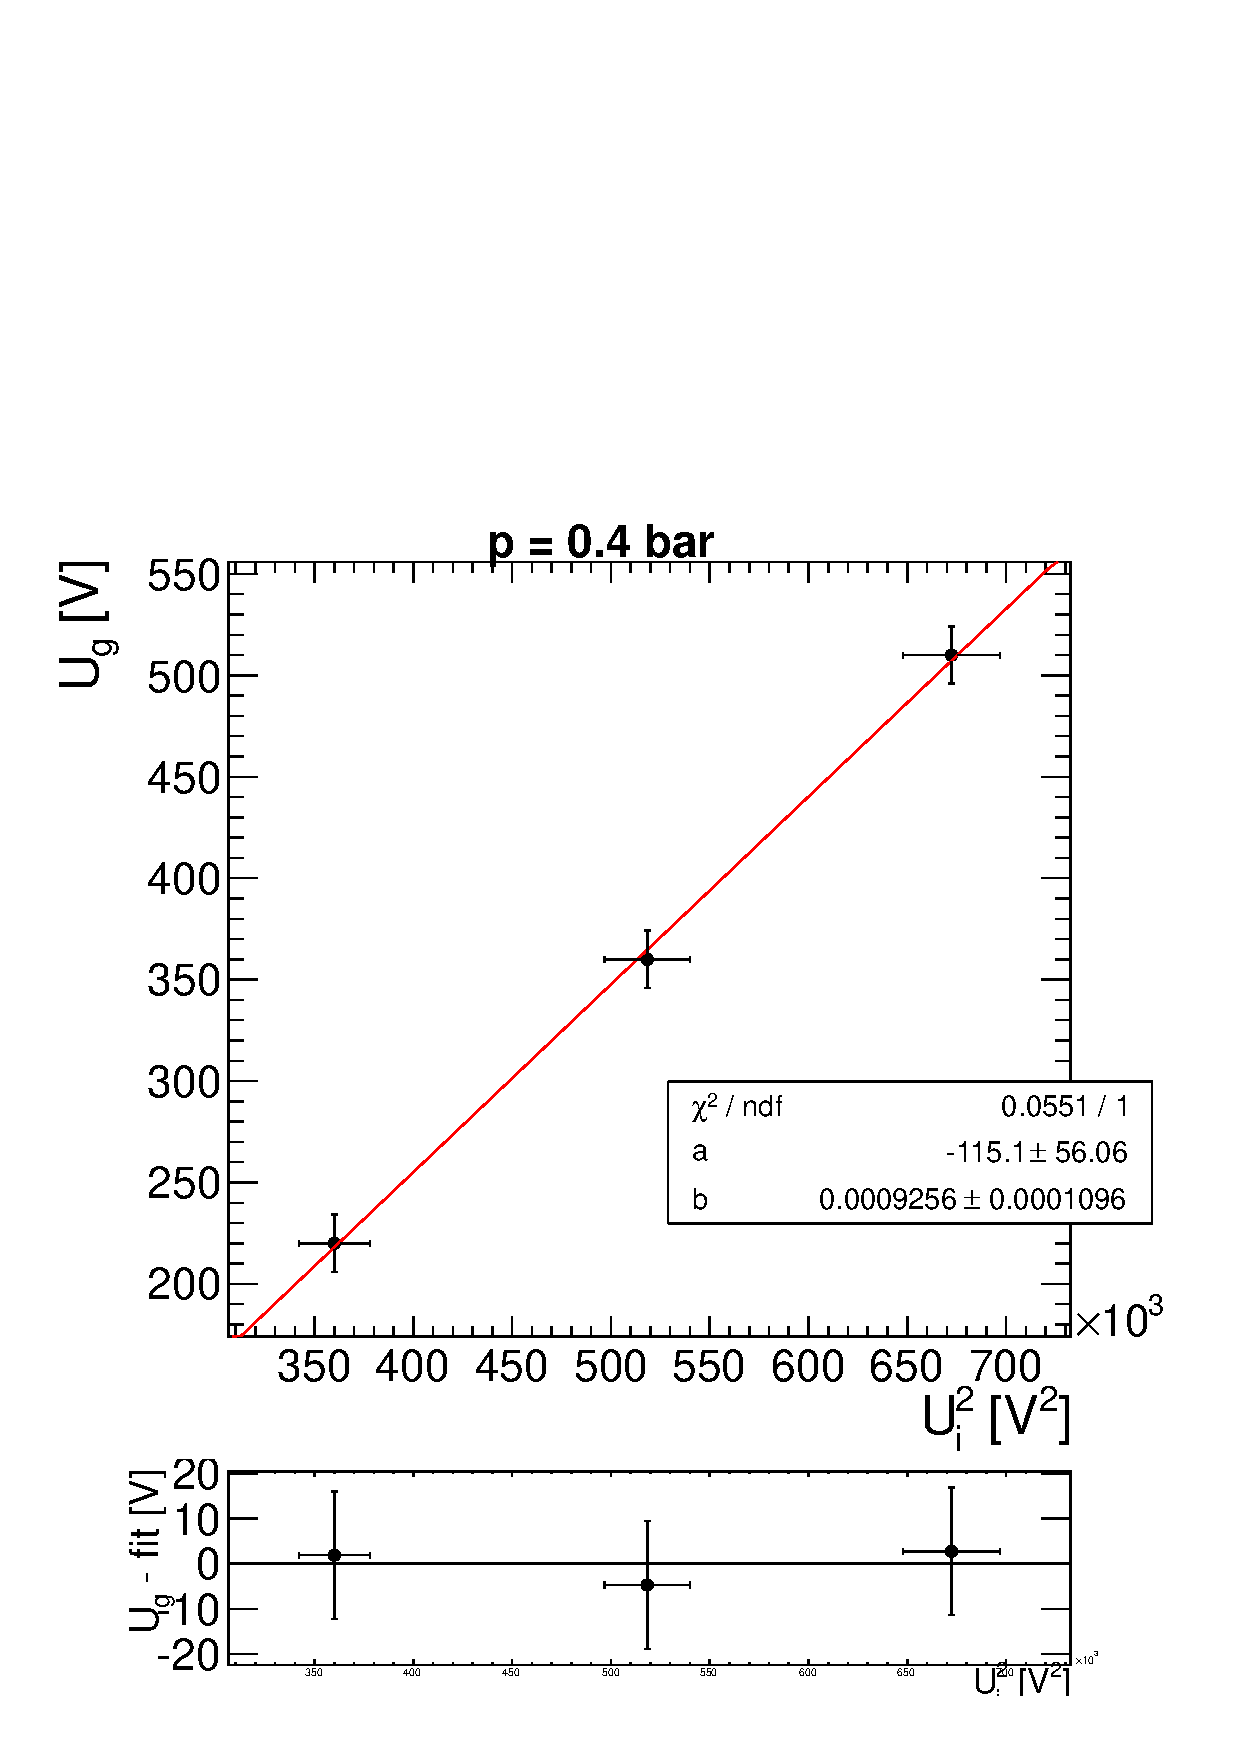
\includegraphics[height = 0.3\textheight]{linReg400bar.pdf}
		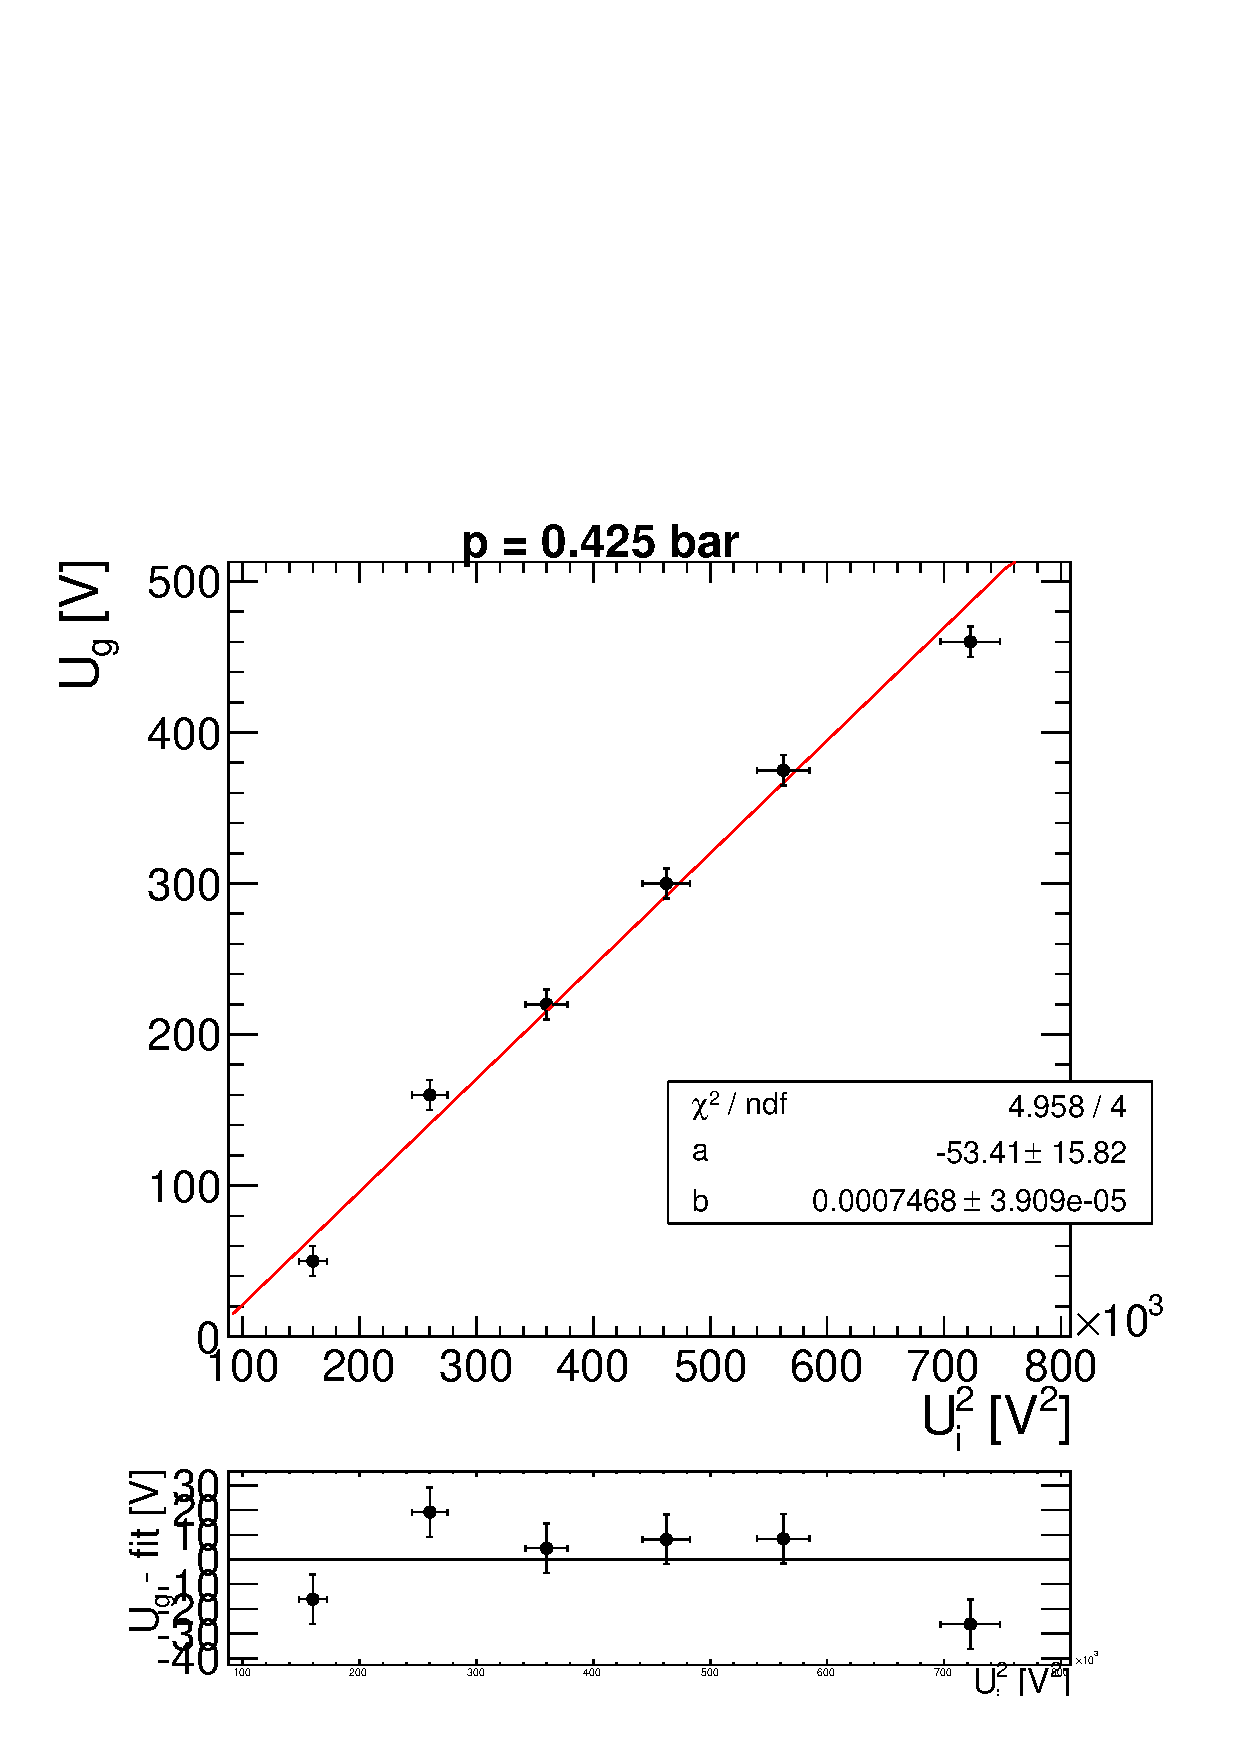
\includegraphics[height = 0.3\textheight]{linReg425bar2.pdf}\\
		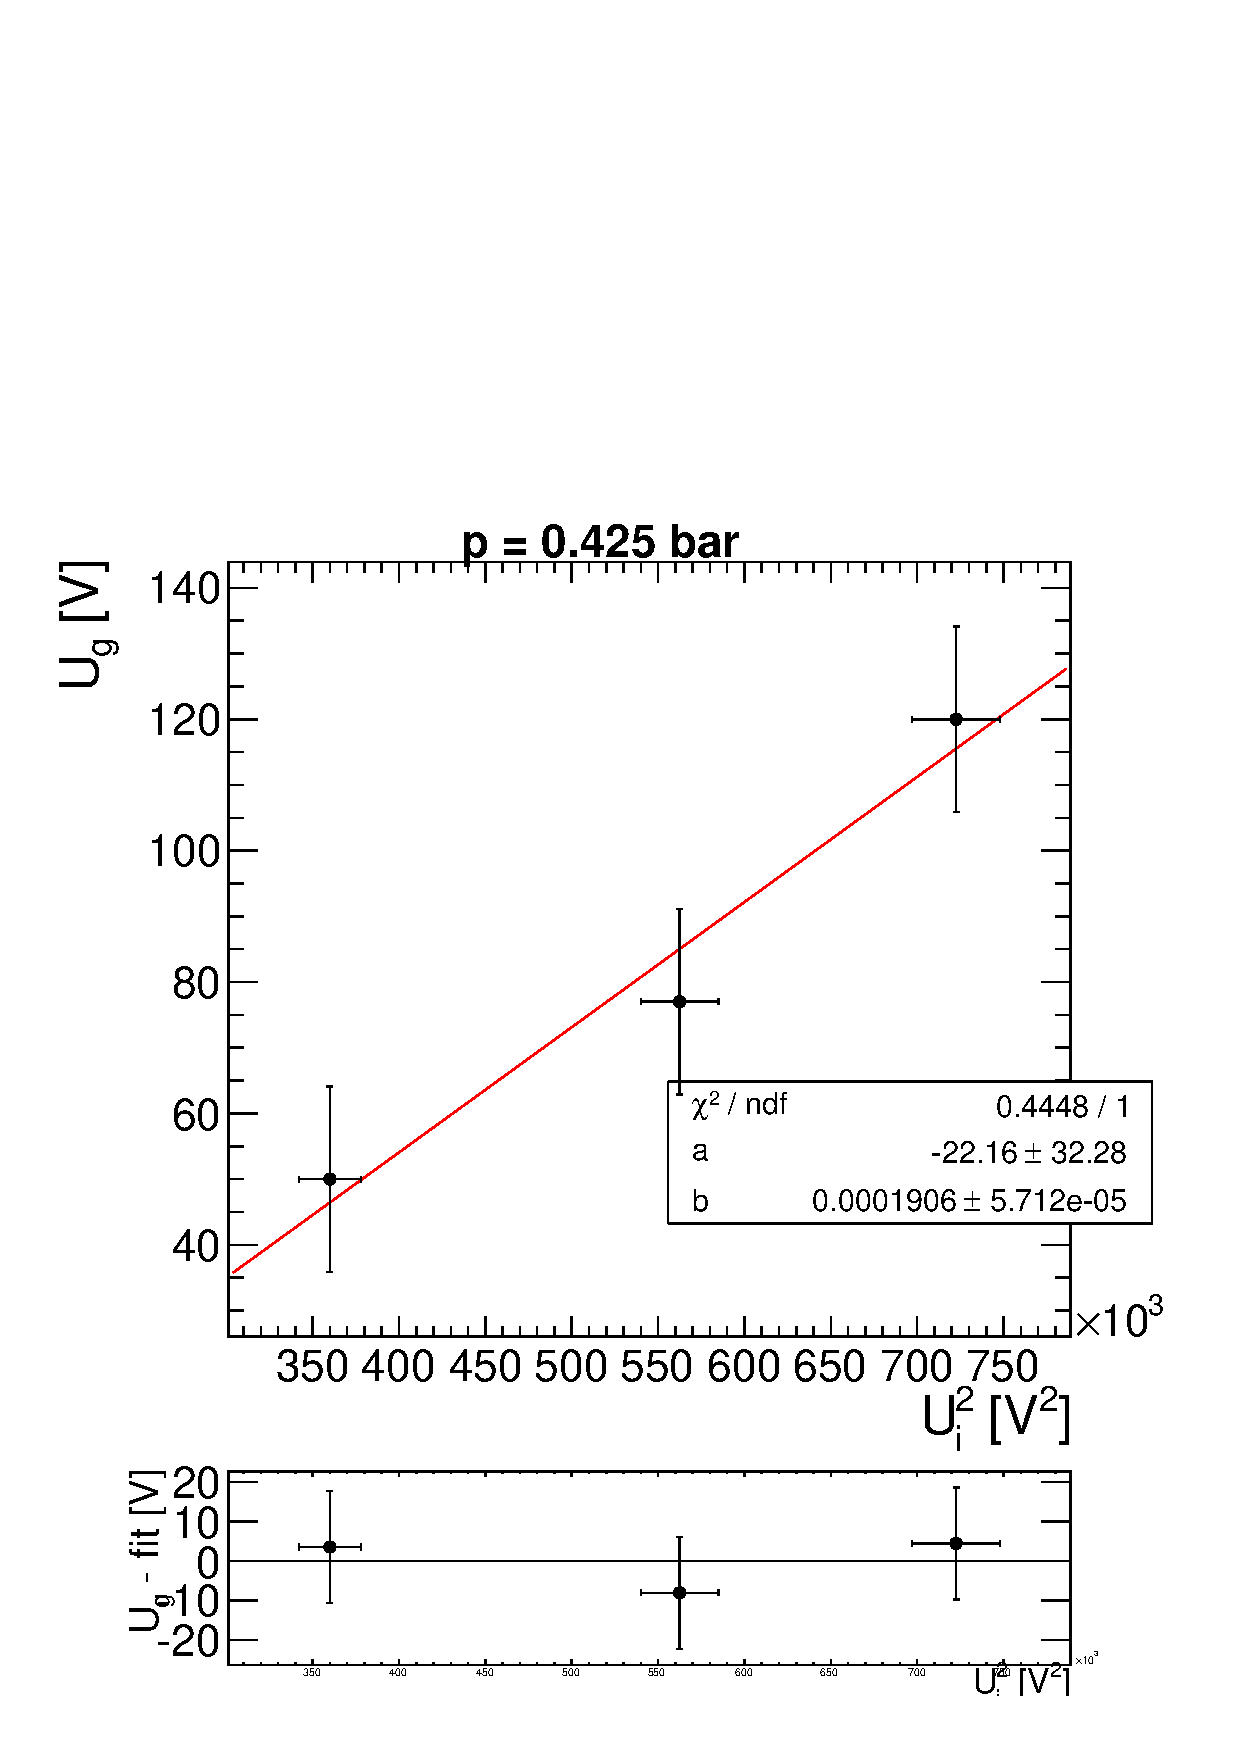
\includegraphics[height = 0.3\textheight]{linReg425bar.pdf}
		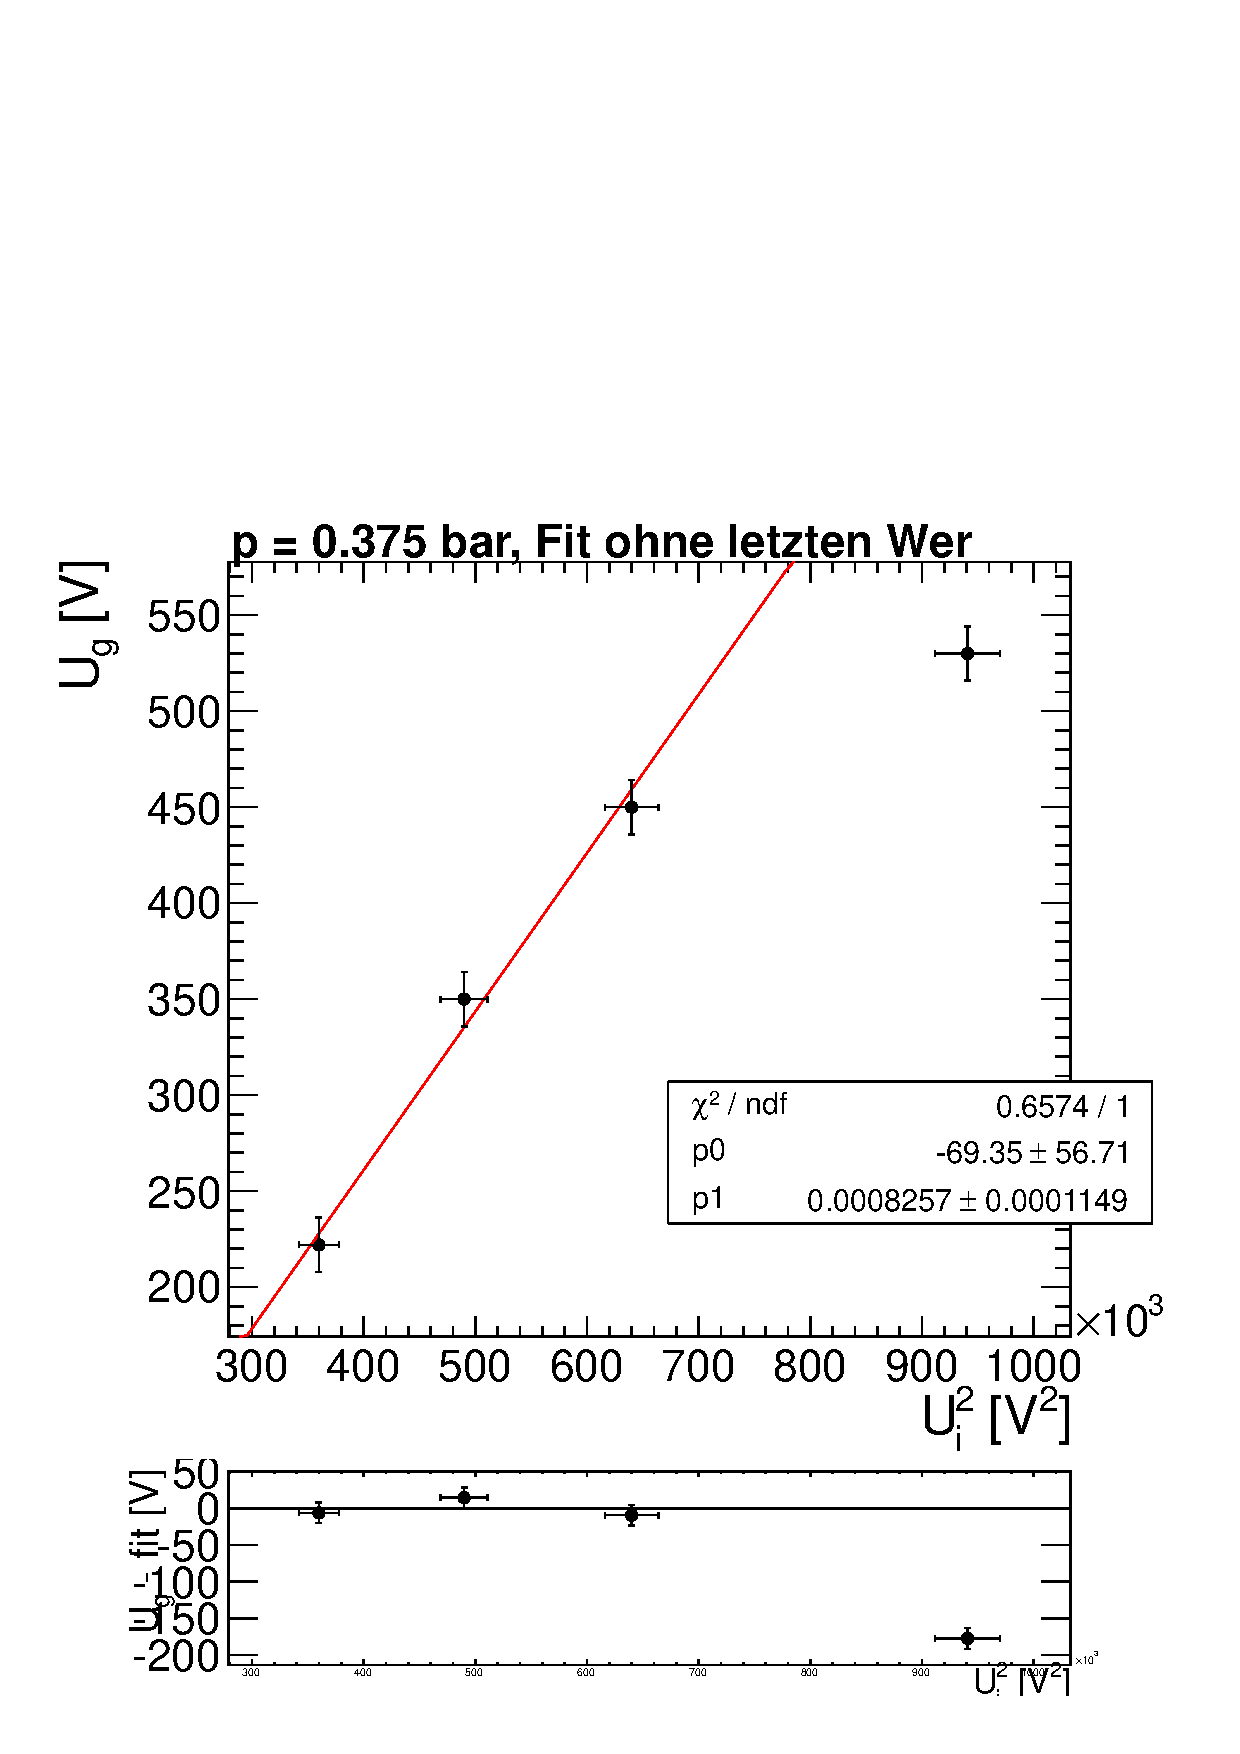
\includegraphics[height = 0.3\textheight]{linReg375bar.pdf}
		\caption{Lineare Regressionen und Residuen zur Stabilitätsuntersuchung für unterschiedliche Luftdrücke und Teilchen.
			Oben links wird der letzte Datenpunkt nicht für die Anpassung benutzt, da das Teilchen die Falle schon verlassen hat.
			Unten rechts wurde die maximale Spannung erreicht, ohne dass die Stabilitätsgrenze erreicht wurde.
		}
		\label{linReg}
\end{figure}

Da der Luftdrucksensor nur $\unit[50]{mbar}$ auflösen konnte, sind die Druckangaben mit einem Fehler von $\unit[14]{mbar}$ behaftet.
Für Messungen, bei denen die Druckanzeige geschwankt hat, wurde der Mittelwert aus beiden Drücken genommen.


Für $U_i$ wird ein Fehler von $\unit[14]{V}$ verwendet, für die Gleichspannung ein Fehler von $\unit[15]{V}$, da sie nicht nur schwankt, sondern auch nur ein geringer Zeitraum zum Ablesen bestand, 
da die Teilchen die Falle schnell verlassen.

In der Anpassung unten rechts wird der letzte Datenpunkt nicht verwendet, da hier die maximale Amplitude der Gleichspannung erreicht wurde.
Das eigentliche Verlassen des Stabilitätsbereichs findet bei einer höheren Spannung statt.
Da durch den genaueren Aufbau der Vakuumfalle besonders viele Teilchen gefangen werden, müssen am Anfang viele Teichen aus dem Stabilitätsbereich gebracht werden, 
damit man die Teichen auseinander halten kann.
Dies führt dazu, dass man nur noch sehr stabile Teilchen in der Falle hat, mit denen man schnell das Maximum der Gleichspannung erreicht.

Wie man schon im Kapitel \ref{sec:kompensation} gesehen hat, sind die Schwankungen von $U_G$ nicht spannungsabhängig.
Dies führt bei kleinen Spannungen zu großen relativen Fehlern, wie man in der Abbildung oben rechts sehen kann.


In der Anpassung oben links wird der letzte Datenpunkt nicht für die Anpassung verwendet, weil bei dem eingestellten Spannungswert das Teichen schon entkommen war.
Man kann über den Abstand des letzen Punktes zur Anpassungsgerade die Spannung abschätzen, die nötig gewesen wäre, ein Teichen tatsächlich aus der Falle zu bringen.
Dies spiegelt sich auch im y-Achsenabschnitt wieder, der im gewichteten Mittel $-\unit[57]{V}$ beträgt und damit mit dem Abstand zur Anpassungsgeraden konsistent ist.
% noch mehr text dazu?
Durch die lineare Regression kann also der systematische Fehler durch das konservative Abschätzen der Entweichspannung verringert werden.


Das $χ^2/ndf$ ist etwas zu klein, besonders an den Graphen, die nur Messwerte bei niedriger Gleichspannung beinhalten, da wie oben beschrieben der relative Fehler hier größer wird.
Die Fehler wurden also zu konservativ abgeschätzt.
Insgesamt sind die Anpassungen gut mit einer Geraden vereinbar.


Über die Steigung der Anpassungsgeraden $b$ kann nun das Verhältnis von Ladung zu Masse ausgerechnet werden:
\begin{align*}
	U_G = -\frac{3K}{2Ω^2r_0^2}\frac{q}{m} U_x^2 =: b U_x^2
\end{align*}

\begin{align*}
	\Leftrightarrow \frac{q}{m} = -\frac{2Ω^2r_0² b}{3K}.
\end{align*}
Die Ergebnisse sind in Tabelle \ref{tab:stabil-result} eingetragen.
In den statistischen Fehler geht der Fehler der Steigung ein, in den systematischen die Unsicherheiten von $Ω$ und $r_0$.
Der Hauptanteil des systematischen Fehlers kommt von der niedrigen Frequnez, mit der der Versuch betrieben wird.
Bei höheren Frequenzen wäre der relative Fehler kleiner, dafür wäre es schwieriger, Teilchen zu fangen.

\begin{table}[h]
	\centering
	\begin{tabular}{ c| c }
		$p [\unit{mbar}]$ & $-\frac{q}{m}[\frac{\mu C}{kg}]$ \\
		\hline
		1000 & 201 ± 20 (stat.) ± 14 (sys.)\\
		1000 & 40 ± 27 (stat.) ± 3 (sys.)\\
		375 & 569 ± 79 (stat.) ± 39 (sys.)\\
		400 & 637 ± 75 (stat.) ± 43 (sys.)\\
		425 & 131 ± 39 (stat.) ± 9 (sys.)\\
		425 & 509 ± 31 (stat.) ± 35 (sys.)
	\end{tabular}
\caption{Das Verhältnis von Ladung zu Masse von verschiedenen Teichen bei verschiedenen Drücken, bestimmt durch die Stabilitätsgrenze}
\label{tab:stabil-result}
\end{table}
Statistische und systematische Fehler sind ungefähr in der gleichen Größenordnung und steigen mit den Werten, was zu etwa konstanten relativen Fehlern führt.

Man sieht keinen Zusammenhang zwischen Druck und dem Verhältnisses von Ladung zu Masse, was daran liegt, dass der Druck nicht niedrig genug war.
Auch die Werte bei gleichen oder ähnlichen Drücken sind nicht vereinbar, was wahrscheinlich damit zu erklären ist, dass die Ladung oder die Masse nicht genau festgelegt ist 
oder die Fehler zu klein abgeschätzt wurden.




\section{Vergleich der Messungen}
Die drei genutzten Messmethoden liefern im Rahmen ihrer Fehler inkompatible Ergebnisse. Die Messwerte für $\frac{q}{m}$ unterscheiden sich deutlich um mehrere Größenordnungen:
\begin{table}[h]
	\centering
	\begin{tabular}{lr}
		Z Kompensation  & $\approx \unitfrac[ 1 ]{mC}{kg}$\\
		Resonanz & $\approx \unitfrac[ 0.1 ]{mC}{kg}$\\
		Stabilität &  $\approx \unitfrac[ 0.001-0.01 ]{mC}{kg}$\\
	\end{tabular}
	\label{result_compare}
\end{table}
%Mögliche Gründe ?
Es ist dabei zu beachten, dass die einzelnen Messungen, die mit einer Messmethode durchgeführt wurden, innerhalb ihrer Fehler
mit einander kompatibel sind.
Für die beobachteten Unterschiede gibt es zunächst zwei Erklärungsansätzte:
Entweder befinden sich alle Teilchen in einem begrenzten $\frac{q}{m}$ Bereich und nur eine Methode liefert 
richtige Ergebnisse oder die möglichen Werte für $\frac{q}{m}$ erstrecken sich über viele Größenordnungen
und jede einzelne Methode eignet sich nur dafür Teilchen aus einem bestimmten Bereich zu vermessen.
Gegen die zweite Hypothese spricht, dass sich die Teilchen im allgemeinen auch bei ausgeschalteter Gleich- bzw. Wechselspannung in ihrer 
Leuchtkraft und dem Verhalten ihrer Bahn unter Veränderung der Fokussierspannung stark ähneln 
sind große Differenzen in $\frac{q}{m}$ unwahrscheinlich. Ein quantitativer Vergleich der Messmethoden hätte nur erfolgen können,
wenn mehrere Messmethoden nacheinander am selben Teilchen durchgeführt werden. Dies ist auf Grund der bereits erwähnten
technischen Problemen im Versuchsaufbau leider nicht möglich gewesen. Die Messungen für $\frac{q}{m}$ bei vermindertem Luftdruck liegen für die 
jeweilige Messmethode in der gleichen Größenordnungen wie die Messungen bei Normaldruck. Es fehlen hier jedoch weitere Messungen, um eine Aussage
über die Auswirkungen der Luftreibung auf die Messung zu bestimmen.

Eine Zusammenfassung aller Ergebnisse ist in Abbildung \ref{final_plot} dargestellt 
( man beachte die Überhöhung der dargestellten Fehler für die Resonanz und Stabilitätsmessung mit einem Faktor von 3).
\begin{figure}[htb]
		\centering
		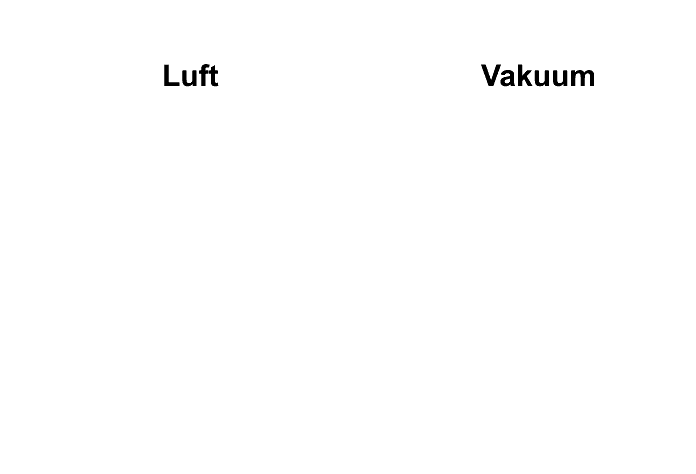
\includegraphics[height = 0.8\textwidth]{../analyse/final_plot.pdf}\\
		\caption{Zusammenfassung der Ergebnisse in logarithmische Auftragung, die Darstellung der Fehler für Stabilität und Resonanz wurden mit 3 multipliziert}
		\label{final_plot}
\end{figure}



\section{Fazit}
Die Versuchsdurchführung war dadurch geprägt, dass die Spannungsquelle nur stark schwankende Ausgangsspannungen geliefert hat. Besonders ein regelmäßiges plötzliches Abfallen der Fokussierspannung 
für ein Flächenpaar hat zu regelmäßigem Verlust der Teilchen geführt. Insbesondere die Resonanzmessung und die Stabiliätsmessung waren oft nicht durchzuführen, weil ein langfristiges Einfangen der Teilchen 
nicht möglich war. Ein quantitativer Vergleich der Messmethoden kann auf Grund dieser ungleichmäßigen Messbedingungen nicht durchgeführt werden. 

\bibliographystyle{plain}
\bibliography{citebib}{}

\end{document}
